\documentclass[10pt]{report}

%##############################################################################%
% PACKAGES %
%##############################################################################%

%% FONTS %%
%\usepackage[light,math]{iwona}
%\usepackage[T1]{fontenc}
%\usepackage{newcent}
\usepackage[sc]{mathpazo}
%\usepackage{helvet}

%% MATH %%
\usepackage{amsmath,amsfonts,amssymb}   % maths typing enhancements
\usepackage{array}
\usepackage[range-units=single]{siunitx}
\usepackage{mhchem}

%% FORMATTING %%
\usepackage{fancyhdr}                   % customisation of page headers and footers
\usepackage[sf,bf]{titlesec}
\usepackage{datetime}
\usepackage{color}
\usepackage[small,bf,hang,font=sf]{caption}     % fancy captions
\usepackage[hidelinks]{hyperref}
\usepackage[xetex]{graphicx}
\usepackage{subcaption}
\usepackage{bm}
\usepackage{setspace}
\usepackage[a4paper,inner=4.0cm,outer=2.5cm,top=2.5cm,bottom=4cm]{geometry}
%\usepackage{epigraph}

%% FIXES %%
\usepackage{fixltx2e}                   % use \textsubscript and other fixes
\usepackage[capitalise]{cleveref}

%% CUSTOM COMMANDS ETC. %%
\usepackage{mystyle}

%##############################################################################%
% DOCUMENT %
%##############################################################################%

\begin{document}

%% TITLE PAGE %%
\thispagestyle{empty}
\begin{center}

%    \newgeometry{top=1cm,bottom=1cm,outer=1cm,inner=1cm}
    \rule{10cm}{0.5mm}

    \huge
    {\sc
        Ab Initio Modelling of \\
        Photoinduced Electron Dynamics \\
        in Nanostructures 
    }

    \vspace{-0.5cm}
    \rule{10cm}{0.5mm}

    \vspace{1.5cm}
    \Large 
    A Thesis \\[0.5cm]
    Presented Upon Application for \\
    Admission to the Degree of \\[0.5cm]

    \LARGE
    {\sc Doctor of Philosophy} \\[0.5cm]

    \Large 
    in the\\
    Faculty of Engineering and Physical Sciences\\[0.5cm]
    by \\[0.2cm]

    \LARGE
    \textbf{Ryan J. McMillan} \\
    MSci (Hons) 2013 \\[0.7cm]

    
\includegraphics[height=4cm]{img/QUB.eps}

    \vspace{0.5cm}
    \Large
        School of Mathematics and Physics\\
        Queen's University Belfast\\
        Northern Ireland\\[0.5cm]
    
    \LARGE
    \monthyeardate\today

    \normalsize
\end{center}

%%

\pagenumbering{roman}
\setstretch{1.5}

%% TABLE OF CONTENTS %%
\clearpage
\tableofcontents

%% LIST OF FIGURES %%
\clearpage
\listoffigures
%%

\pagenumbering{arabic}
\setlength{\topmargin}{0.4cm}
\setlength{\headsep}{0.6cm}

%% INTRO %%
\clearpage
\chapter{Background and Introduction}


\section{Motivation - Solar Technology}

\section{2D Materials in Photonics}\label{sec:2d}

\section{Increasing Light Absorption in 2D Materials}\label{sec:light_2d}

%%

%% THEORY %%
\clearpage
\chapter{Theory}


\section{Background Theory}\label{sec:background_theory}

\subsection{Electronic Structure Calculations}\label{sec:elec_struc}

\subsection{Excited State Calculations}\label{sec:ex_state}

\subsection{Obtaining Optical Properties}\label{sec:opt_prop}


%\section[Projected Equations of Motion (PEOM) Method for Semiconductor-Metal Composites]{Projected Equations of Motion (PEOM) Method for\\ {Semiconductor-Metal} Composites}\label{sec:peom}
\section{Projected Equations of Motion (PEOM) Method for\\ {Semiconductor-Metal} Composites}\label{sec:peom}

The efficiency of a PV device is largely determined by its ability to absorb
light. We mentioned in \cref{sec:light_2d} that the performance of 2D,
TMD-based solar cells may be improved by depositing MNPs on the TMD monolayer.
In the presence of light, the MNPs enhance the field near the monolayer which
in turn increases its light absorption.

The absorption in the monolayer may be obtained theoretically using the methods
described in \cref{sec:background_theory}. For example, to calculate the
absorption in a monolayer of \ce{MoS2}, one would first perform a DFT calculation on
a unit cell (containing three atoms) to determine the ground state electronic
configuration. A linear response TDDFT calculation could then be carried out
and the optical absorption spectrum obtained. Such calculations are routine and
can be easily completed on a modern desktop computer in a relatively short
period of time. Suppose we now wish to perform a similar calculation for an
\ce{MoS2} monolayer decorated with gold nanoparticles of diameter
\SI{15}{\nano\metre}, similar to the system studied experimentally in
Ref.~\cite{Lin2013}. In this case, one
must construct a supercell containing around \num{50000} times more atoms and
having a volume greater than \num{100000} times that of the original unit
cell of the bare \ce{MoS2} monolayer. Such a calculation at the DFT level would
prove extremely demanding: even with a
linearly scaling code running on many cores of a supercomputer, the
boundaries on computational resources are being pushed if not exceeded.
Moreover, the calculation becomes infeasible if one
wishes to model excitonic effects using, for example, the Bethe-Salpeter
Equation as described in
~\cref{sec:background_theory}.

For this system, however, we are interested primarily with the optical response
of the \ce{MoS2} monolayer as it is the `active' component of the PV device. The MNP
on the other hand contributes just to modify the optical properties of the
monolayer. Due to the large difference in scale of the MNP compared to the
monolayer (in terms of the unit cells required for the DFT calculations), it
may then be appropriate to model the MNP on a level of theory less
computationally demanding than DFT and to couple the dynamics to those of the
monolayer by some effective method. 

Indeed, similar problems occur in other areas of computational chemistry and
various hybrid methods have been used to great effect over the past few
decades. For example, the quantum mechanics/molecular mechanics (QM/MM)
approach has been widely applied to study chemical reactions in large systems.
In the QM/MM method, the larger environment (e.g. a solvent) is treated on the
basis of classical molecular mechanics while the smaller system of interest
(e.g. a molecule) is treated using a quantum approach (e.g. DFT). The two
systems can then be coupled via force fields or electrostatically as in the
polarizable continuum model.

In Ref.~\cite{Zhang2006} a method is developed for modelling the interaction
between a semiconducting quantum dot (SQD) and an MNP under illumination. In
this case, the SQD is treated as a two-level atomic-like system using the
density matrix formalism of quantum mechanics while the MNP is modelled using
classical electrodynamics. The dynamics of the two systems are then coupled
through the externally applied field using a dipole-dipole approximation. The
dynamics of this hybrid complex can be solved analytically within the so-called
rotating wave approximation (RWA) as described in detail in \cref{app:sqd-mnp}. This
analytical solution is valid provided the applied field is a slowly-varying
monochromatic pulse of frequency close to the frequency gap of the SQD.
Moreover, the optical response function of the MNP is assumed to be much
broader than that of the SQD which is inherently narrow due to its two-level
nature and relatively long dephasing times. As it stands, the solution will not
hold for ultrafast pulse excitation which is an area of current interest for
such systems. Moreover, if the SQD is replaced with a semiconducting monolayer,
the two-level quantum description will not suffice and the profile of the
MNP response function can no longer be considered `broad'. Therefore, the method
should be generalised to lift the restrictive approximations commonly used,
giving rise to the proposed project equations of motion (PEOM) approach
described in this section. 

\begin{figure}[ht]
    \centering
    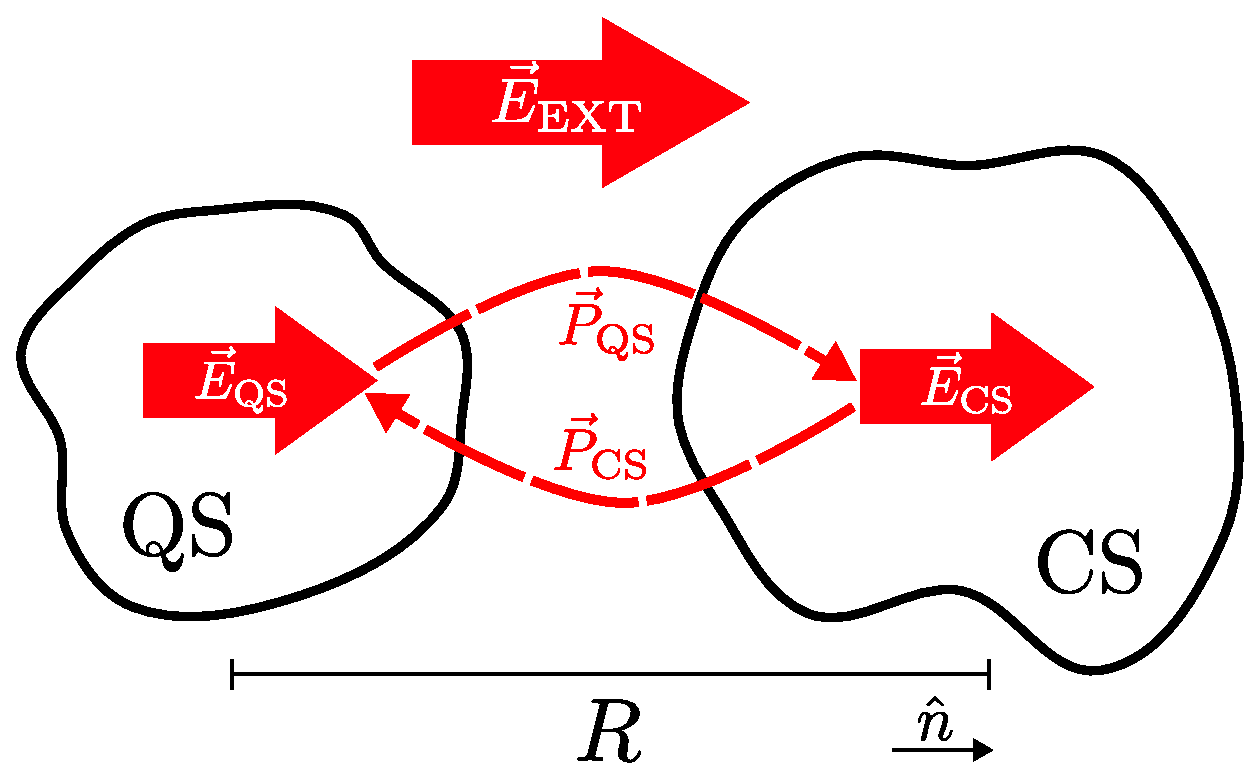
\includegraphics[width=0.6\columnwidth]{img/qs-cs.eps}
    \caption{Schematic diagram showing the dipole-dipole interaction between a
        QS and a CS, separated by a distance $R$.  When an external field,
        $\veext$, is applied, a dipole moment, $\vpqs$, is induced in the QS,
        generating a field. The CS thus experiences this dipole field in
        addition to the external field, and we denote the total field felt by
        the CS as $\vecs$. Similarly, due to $\vecs$, a dipole field is
        generated in the CS which is in turn felt by the QS in addition to
        $\veext$, and we denote the total field felt by the QS as $\veqs$. In
    this way, the QS and CS dynamics are coupled through the external field.}
    \label{fig:qs-cs}
\end{figure}

\note{[Would the terms ``primary system'' and ``auxiliary system''
describe the setup better?]} In order to introduce the PEOM method, 
we consider a general composite comprising two, isolated subsystems in a vacuum:
a larger system to be treated
classically---the classical system (CS)---and a smaller system of interest to
be treated on the basis of quantum mechanics---the quantum system (QS). For
example, in the semiconducting monolayer-MNP system, the monolayer would be the
QS and the MNP the CS. The QS and CS shall be separated by some distance, $R$.
An external field, $\veext(t)$, is applied which induces a dipole-dipole
interaction between the two systems as described in \cref{fig:qs-cs}.
To simplify the
notation, we assume that the QS and CS are isotropic media. For the
generalization to the anisotropic case see \cref{app:anis}.
We write
$\veext(t)\equiv\eext(t)\ve$ and denote the unit vector pointing along the
line separating the centres of the systems as $\hat n$. The fields felt by
the QS and CS are then,
respectively~\cite{jackson_classical_1962,schmitt_preparation_1999,zhang_semiconductor-metal_2006},
\note{(note that I've removed the background dielectric constant, $\epsb$, as I
only ever use a vacuum and it simplifies notation.)}
%
\begin{subequations}
    \begin{align}
        \veqs(t) &= \eext(t)\ve + \frac{\pcs(t)}{\epsb R^3}\g \ , \label{eq:eqs}\\
        \vecs(t) &= \eext(t)\ve + \frac{\pqs(t)}{\epsb R^3}\g \ , \label{eq:ecs}
    \end{align}
    \label{eq:fields1}
\end{subequations}
%
where $\pcs(t)$ ($\pqs(t)$) is the total dipole moment of
the CS (QS), and
%
\begin{equation}
    \g=3\hat n\left( \ve \cdot \hat n \right) - \ve \ .
    \label{eq:g_def}
\end{equation}
%
\note{Is this actually correct? I can see that if $\hat n$ is parallel or
perpendicular to $\hat e$ then yes, but what if it's at 45 degrees? Will there
be a dipole along $\hat e$ and $\hat n$ both?\ldots}

The time-dependent dipole moment of the QS, $\pqs(t)$, can be
obtained, e.g., using the methods outlined in Section REF. In general, it is
found by solving some equations of motion, whether they be from the density matrix
master equation (Eq. REF), or the real-time Bethe-Salpeter equation (Eq. REF),
although the theory presented here is independent of the chosen method.

For the CS, rather than calculate the dipole moment explicitly by solving EOMs
from quantum theory (or even from classical electrodynamics), we assume that
its frequency dependent polarizability, $\alpha(\omega)$, is already known.
This may have been previously obtained, however, from \textit{ab-initio}
calculations similar to the QS, or from experimental data or classical
approximations.  Its dipole moment can then be described (in the linear
response regime) via~\footnote{Gaussian units are assumed throughout this
    thesis \note{--THIS SHOULD GO AT THE START SOMEWHERE INSTEAD.}}
%
\begin{equation}
    \vpcs(\omega) = \epsb  \alpha(\omega)\vecs(\omega) \ .
    \label{eq:pcs_omega}
\end{equation}
%
In the time domain, however, the dipole moment
is written in terms of the response function $\alpha(t)$, as
%
\begin{equation}
    \vpcs(t) = \epsb \int_{-\infty}^{t}\alpha(t-t')\vecs(t')dt' \ .
    \label{eq:P_2}
\end{equation}
%
Now, the EOMs that determine $\vpqs(t)$ depend on $\veqs(t)$ which in turn
depends on $\vpcs(t)$ from \cref{eq:eqs}. They are generally solved
using an iterative algorithm, such as the fourth-order Runge-Kutta method (see
\cref{app:runge-kutta} \note{--not sure whether it's necessary to include this
in the appendix\ldots}), where the time domain is split into a set of discrete points.
However, computing the integral in Eq.~\eqref{eq:P_2} at each time-step in the
solution is cumbersome and the values of $\vecs(t)$ and $\alpha(t)$ for each
time-step must be held in memory which may not be feasible for long
simulations.  Moreover, while $\alpha(\omega)$ is known beforehand, $\alpha(t)$
is not and would have to be calculated using, e.g., a discrete fourier
transform. In this case one would have to ensure a sufficiently large
(\note{small?}) time-resolution of the transform in order to match the
time-step in the algorithm used to solve the quantum EOMs. However, the
resolution is limited to whatever data is available for $\alpha(\omega)$.
\note{ Not sure if this last part is necessary, or too confusing. Also,
would this method actually work? I would guess a very small time-step would be
needed\ldots }

In Ref.~\cite{stella_generalized_2014}, a method (originally devised for memory
kernels in the Generalised Langevin Equation) is presented for avoiding the
memory-dependent time-convolution inherent in \cref{eq:P_2}. Inspired by this,
we introduce $N$ complex auxiliary degrees of freedom, $\{\vs_k(t)\}$ which
satisfy the following projected equations of motion (PEOMs)
%
\begin{equation}\label{eq:s_EOM}
    \dot{\vs}_k = -\left( \gamma_k + \imagn\omega_k \right)\vs_k + \imagn\epsb
    \vecs(t)\ \quad \text{for }k=1,2,\ldots,N \
    .
\end{equation}
%
We then state that $\vpcs(t)$ can be written as
%
\begin{equation}\label{eq:P_2_approx}
    \vpcs(t) \approx \sum_{k=1}^{N} c_k \real{\vs_k(t)} \ ,
\end{equation}
%
so that the memory-dependent integral in Eq.~\eqref{eq:P_2} is replaced with an
expansion over the functions $\vs_k$ found by solving the differential
equations in Eq.~\eqref{eq:s_EOM}. As these differential equations no longer
contain a time-convolution (i.e., they are ``memoryless''), they can be
efficiently integrated using, e.g., the same iterative algorithm as for the QS. 
Therefore, the QS EOMs and the CS PEOMs can be efficiently solved in a coupled
fashion.
All that
is required is to find suitable values for the (real) parameters $\{c_k,
\gamma_k, \omega_k\}$ in Eq.~\eqref{eq:s_EOM}.
The formal solution of Eq.~\eqref{eq:s_EOM} is
%
\begin{equation}
    \vs_k(t) = \epsb \int_{-\infty}^{t}\imagn\ e^{-\left( \gamma_k + \imagn\omega_k
    \right)\left( t-t' \right)} \vecs (t') dt' \ .
    \label{eq:s_k}
\end{equation}
%
Substituting the real part of Eq.~\eqref{eq:s_k} into Eq.~\eqref{eq:P_2_approx} and
rearranging yields
%
\begin{equation}
    \vpcs(t) \approx \epsb
    \int_{-\infty}^{t} 
    \left( 
        \sum_{k=1}^{N} c_k e^{-\gamma_k (t-t')}\sin[\omega_k(t-t')]
    \right) 
    \vecs(t') dt' \ ,
\end{equation}
%
and comparing with Eq.~\eqref{eq:P_2} we see that
%
\begin{equation}
    \alpha(t) \approx 
        \sum_{k=1}^{N} c_k e^{-\gamma_k t}\sin(\omega_k t) \ .
    \label{eq:chi_t}
\end{equation}
%
Taking the Fourier transform of
Eq.~\eqref{eq:chi_t} (using the causality condition) gives
%
\begin{equation}
    \alpha(\omega) \approx \sum_{k=1}^{N}\frac{c_k}{2}
    \left[ \frac{1}{\omega+\omega_k +\imagn\gamma_k}
    -\frac{1}{ \omega-\omega_k +\imagn\gamma_k}\right] \ .
    \label{eq:chi_approx}
\end{equation}
%
Hence, the parameters $\{c_k,\gamma_k,\omega_k\}$ may be found by fitting
the frequency-dependent polarizability of the CS (which is known)
to the functions on the RHS of Eq.~\eqref{eq:chi_approx}
(e.g. using the least squares method\note{--in appendix?}).

%%

%% RESULTS %%
\clearpage
\chapter{Results}\label{ch:results}


\section{Semiconducting Quantum Dot-Metal Nanoparticle Hybrid}\label{sec:sqd-mnp}

In order to test the proposed PEOM method detailed in \cref{sec:peom}, we model a
semiconducting quantum dot (SQD) as the quantum \note{(primary)} system and a metal
nanoparticle (MNP) as the classical \note{(auxiliary)} system. The SQD-MNP
hybrid system has been studied extensively both theoretically (REFS) and
experimentally (REFS). In particular, in Ref.~\cite{Zhang2006}, Zhang et al.
introduce a simple theoretical model in which the SQD is treated as a 
two-level, atomic-like quantum system whose dynamics are solved using the
density matrix formalism of quantum mechanics. The MNP on the other hand is
treated classically and the systems' dynamics are coupled through the external
field. Indeed, this method provided the basis for the PEOM method.

For a monochromatic external field, the energy absorption rate of the hybrid
system can be calculated analytically by means of the rotating wave
approximation (RWA). In \cref{sec:en_abs_rates}, we compare examples of these
analytical solutions and show agreement with the PEOM method.

For a pulsed external field, population inversion in the SQD can be obtained
and modified by the presence of the MNP. For slowly-varying pulse envelopes,
the density matrix equations of motion for the SQD can be solved
semi-analytically within the RWA and in \cref{sec:pop_inv}, we show agreement
with the PEOM method for picosecond pulses. However, in the case of ultrafast,
femtosecond pulses, we show that the RWA breaks down and the PEOM method must
be preferred for more accurate results.

\subsection{Describing the System}\label{sec:sqd-mnp_setup}

\begin{figure}[ht]
    \centering
    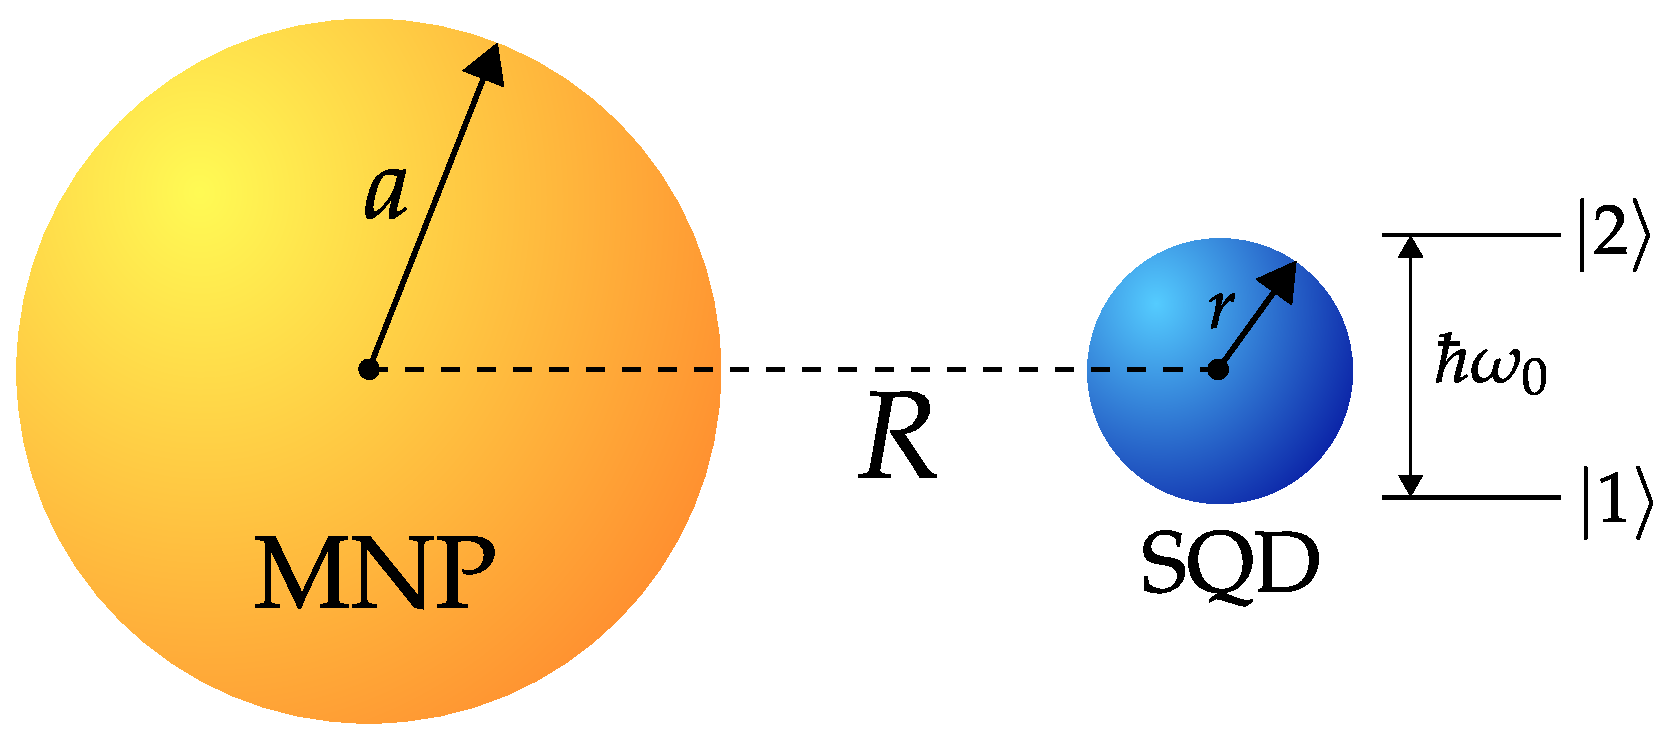
\includegraphics[width=0.8\textwidth]{sqd_mnp_schem.eps}
    \caption{Schematic diagram of a spherical metal nanoparticle (MNP) of
        radius, $a$, separated by a distance, $R$, from a spherical
        semiconducting quantum dot (SQD) of radius, $r$.  The MNP is modelled
        classically while the SQD is treated as a two-level quantum system with
        ground state, $\state{1}$, and excited state, $\state{2}$, separated by
    an energy gap of $\hbar\omega_0$.}
    \label{fig:sqd-mnp_scem}
\end{figure}

\noindent Consider a spherical, gold MNP of radius, $a$, separated by a distance,
$R$, from a spherical
SQD of radius, $r$, as shown in \cref{fig:sqd-mnp_scem}.
From \cref{eq:fields1}, when an external field $\eext(t)$ is applied, the
fields felt by the SQD and MNP are, respectively,
%
\begin{align}
    \esqd(t) &= \eext(t) + g\frac{\pmnp(t)}{\epsb R^3} \ , \label{eq:esqd}\\
    \emnp(t) &= \eext(t) + g\frac{\psqd(t)}{\epsb R^3} \ ,
\end{align}
%
where $\psqd(t)$ ($\pmnp(t)$) is the dipole moment of the SQD (MNP).
We have taken the external field to be polarized along the line connecting the
centres of the particles so that $\hat n=\hat e$. From \cref{eq:g_def}, we have
that $\vec{g}=2\hat e$ and so all fields are pointing in the direction of the
external field, $\hat e$, allowing us to drop the vector notation.

The SQD is treated as a 2-level, atomic-like system with ground state,
$\state{1}$, and excited state, $\state{2}$, separated by an energy gap of
$\hbar\omega_0$ ($\omega_0$ is known as the exciton frequency). We use the
density matrix formalism so that the SQD can be described by a $2\times
2$ density matrix, $\bm\rho(t)$, whose elements can be written as (see Appendix
REF\note{(--from differentiation)})
%
\begin{equation}
    \begin{cases}
        \dot{\Delta} &= -\frac{4\mut}{\hbar}\esqd(t)\imag{\rho_{21}} -
        \Gamma_{11}(\Delta - 1)   \\
        \dot\rho_{21} &= -\left( \Gamma_{21}+\imagn\omega_0
        \right)\rho_{21} + \imagn\frac{\mut}{\hbar}\esqd(t) \Delta
        \label{eq:eoms}
    \end{cases} \ ,
\end{equation}
%
where $\Delta(t)=\rho_{11}(t)-\rho_{22}(t)$ is the population difference between the
ground and excited states, and $\rho_{12}=\rho_{21}^*$. $\Gamma_{11}$ and $\Gamma_{21}$ are the population
decay and dephasing rates of the system respectively. The SQD is assumed to be
a
dielectric sphere with dielectric constant $\epss$ and so it has a screened
dipole matrix element,
%
\begin{equation}
    \mut=\frac{\mu_{21}}{\epseff} \ ,
\end{equation}
%
where $\mu_{21}$ is the bare
dipole matrix element and~\cite{batygin_problems_1978}
%
\begin{equation}
    \epseff=\frac{2\epsb+\epss}{3\epsb} \ .
\end{equation}
%
\note{(Not sure if these should go here or later\dots)} We take the SQD system parameters from
Ref.~\cite{zhang_semiconductor-metal_2006}, which are typical of a \ce{CdSe}
quantum dot.
The dielectric
constant is taken to be $\epss=6$ with (bare) transition dipole moment $\mu=0.65e$~nm and
exciton energy $\hbar\omega_0=2.5$~eV close to the plasmon peak of the gold MNP.
The decay and dephasing times are given by
$\Gamma_{11}^{-1}=0.8$~ns and $\Gamma_{21}^{-1}=0.3$~ns. 

The dipole moment of the SQD is
%
\begin{align}
    \psqd(t) &= \trace{\bm\rho\bm\mu} \\
    &= \mut\left( \rho_{12} + \rho_{21} \right) ,
    \label{eq:psqdt}
\end{align}
%
where $\trace{\cdots}$ is the matrix trace operator. The dipole moment of the
MNP is taken to be
%
\begin{equation}
    \pmnp(\omega) = \alphamnp(\omega)\emnp(\omega) \ ,
    \label{eq:pmnpw}
\end{equation}
%
where $\alphamnp(\omega)$ is the frequency-dependent polarizability.
For comparison with previous literature, we approximate $\alphamnp(\omega)$ by
the Clausius-Mossotti formula,
%
\begin{equation}
    \alphamnp(\omega) = a^3 \frac{\epsm(\omega)-1\epsb}{
    \epsm(\omega) + 2\epsb} \ ,
    \label{eq:alpha_mnp}
\end{equation}
%
where $\epsm(\omega)$ is the frequency-dependent dielectric function of the
bulk metal~\cite{landau_electrodynamics_1984} (we use the analytical model for
bulk gold as given by Etchegoin et al.~\cite{etchegoin_analytic_2006}).

For the external field, we shall consider the following light pulse,
%
\begin{equation}
    \eext(t) = f(t) E_0 \cos(\omega_L t) \ ,
    \label{eq:pulse_general}
\end{equation}
%
where $f(t)$ is a dimensionless pulse envelope, $\omega_L$ is the carrier (or
central) frequency and $E_0$ is the amplitude. The field strength is normally
given in terms of the intensity, $I_0$, by
%
\begin{equation}
    I_0 = \frac{c}{2}E_0^2 \ ,
    \label{eq:intensity}
\end{equation}
%
where $c$ is the speed of light. \note{$I_0=\frac{\epsilon_0 c}{2}E_0^2$, in
gaussian units, does the $\epsilon_0$ (vacuum permittivity) just disappear, or
should there be a $4\pi$ in there?\ldots}

To determine the solutions to \cref{eq:eoms}, one can (i) follow the PEOM
method in ~\cref{sec:peom}, or (ii) use analytical approximations. We shall now
describe both procedures.

\subsection{Solution within the PEOM Method}\label{sec:sqd-peom}

In the PEOM method, we approximate the time-dependent dipole moment of the
MNP by
%
\begin{equation}
    \pmnp(t) \approx \sum_{k=1}^{N}c_k\real{s_k(t)} \ ,
    \label{eq:pmnpt_peom}
\end{equation}
%
where the functions, $\{s_k\}$, are found by solving the differential
equations,
%
\begin{equation}
    \dot{s}_k = -\left( \gamma_k + \imagn\omega_k \right)s_k + \imagn\epsb
    \emnp(t)\ \quad \text{for }k=1,2,\ldots,N \
    .
    \label{eq:s_k_mnp}
\end{equation}
%
The first step in the implementation, therefore, is to determine the paramters,
$\{c_k,\omega_k,\gamma_k\}$, by fitting the frequency-dependent
polarizability of the MNP, $\alphamnp(\omega)$, to
%
\begin{equation}
    \alphamnp(\omega) \approx \sum_{k=1}^{N}\frac{c_k}{2}
    \left[ \frac{1}{\omega+\omega_k +\imagn\gamma_k}
    -\frac{1}{ \omega-\omega_k +\imagn\gamma_k}\right] \ .
    \label{eq:alphamnp_approx}
\end{equation}
%
The polarizability
for the gold MNP from \cref{eq:alpha_mnp} is shown in \cref{fig:alpha_approx} along with a least-squares
fit to \cref{eq:alphamnp_approx} which required $N=$~\num{21} fitting functions in order to get a fit of
sufficient accuracy over the range \SIrange{0}{10}{\electronvolt}. The
parameters obtained are given in Appendix REF \note{Should I include these in
the appendix?}.

\begin{figure}[ht]
    \centering
    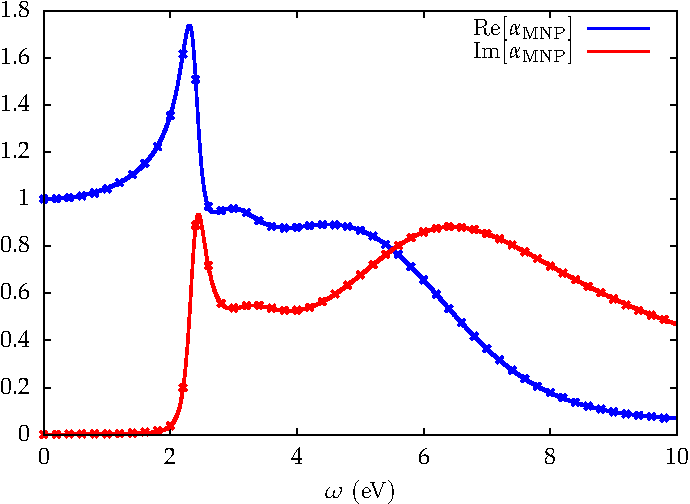
\includegraphics[width=0.8\textwidth]{alpha_mnp_approx.pdf}
    \caption{Real (solid blue) and imaginary (solid red) parts of the MNP
        frequency-dependent polarizability, $\alphamnp(\omega)$, as
        given by \cref{eq:alpha_mnp}. The least-squares fit is shown as
        crosses, obtained from \cref{eq:alphamnp_approx} with
        $N=$~\num{21}. The units of the $y$-axis are in $1/a^3$ where $a$ is the radius of
the MNP.}
    \label{fig:alpha_approx}
\end{figure}

Once the parameters are known, we can then solve \cref{eq:eoms} simultaneously
with \eqref{eq:s_k_mnp} using the fourth-order
Runge-Kutta method (\cref{app:runge-kutta}) where at the end of each step
$\pmnp(t)$ and $\psqd(t)$ are updated using \cref{eq:pmnpt_peom,eq:psqdt}
resepectively.  \note{(Should I include code/pseudo code of the algorithm in
the Appendix?)}.

\subsection{Analytical and Semi-Analytical Solutions}\label{sec:sqd-anal}

To solve \cref{eq:eoms} analytically, we first separate out the slowly and quickly oscillating terms of the
off-diagonal density matrix elements:
%
\begin{subequations}
    \begin{align}
        \rho_{12}(t) = \bar\rho_{12}(t)e^{\imagn\omega_L t} \ , \\
        \rho_{21}(t) = \bar\rho_{21}(t)e^{-\imagn\omega_L t} \ , 
    \end{align}
    \label{eq:rhobar}
\end{subequations}
%
where $\bar\rho_{12}(t)$ and $\bar\rho_{21}(t)$ are assumed to vary much larger
timescale than $2\pi/\omega_L$. We assume a {\it slowly-varying} pulse
envelope so that $f(t)$ also varies on a timescale larger that $2\pi/\omega_L$.
Thus, from \cref{eq:esqd}, we can express the field felt by the SQD
approximately as (see Appendix REF)
%
\begin{equation}
    \esqdeff(t) = \frac{\hbar}{\mut}\left[ \left( \frac{\Omega(t)}{2}e^{-\imagn\omega_L t} +
    G\rho_{21}(t) \right) + \text{c.c.} \right] ,
    \label{eq:effective_field}
\end{equation}
%
where
%
\begin{subequations}
    \begin{align}
        \Omega(t) &= f(t) \omegaeff \ , \label{eq:omega} \\
        \omegaeff &=  \Omega_0 \left[ 1 +
        \frac{g}{R^3}\alphamnp(\omega_L) \right] \ ,\label{eq:omegaeff}\\
        G &= \frac{g^2\mut^2 }{\hbar\epsb R^6}\alphamnp(\omega_L) \ , \label{eq:G}
    \end{align}
\end{subequations}
%
where
%
\begin{equation}
    \Omega_0 = \mut E_0/\hbar 
    \label{eq:omega_0}
\end{equation}
%
is the Rabi frequency of the isolated SQD.

One may then substitute \cref{eq:effective_field} into the density matrix EOMs
in \cref{eq:eoms} and determine a numerical solution (e.g. using the
fourth-order Runge-Kutta method). This is equivalent to the method used by Yang
et al. in REF. Alternatively, one can make use of the rotating wave
approximation (RWA) which assumes that the carrier frequency is close to
resonant with the exciton frequency ($\omega_L\approx\omega_0$) so that terms
oscillating at frequencies far from $\omega_0$ can be neglected. By
substituting \cref{eq:effective_field} into \cref{eq:eoms} and employing the RWA,
one arrives at the following, modified RWA EOMs for the density matrix (see
Appendix REF)
%
\begin{equation}
    \begin{cases}
        \dot\Delta &= 4\imag{\left( \frac{\Omega}{2}+G\bar\rho_{21} \right)\bar\rho_{12}}
        + \Gamma_{11}\left( 1-\Delta \right) \\
        \dot{\bar\rho}_{21} &= \left[ \imagn\left( \omega_L-\omega_0 +G\Delta
        \right)-\Gamma_{21} \right]\bar\rho_{21} + \imagn\frac{\Omega}{2}\Delta 
    \label{eq:eoms_rwa}
    \end{cases}
    \ .
\end{equation}
%
One can then numerically solve these modified EOMs to determine the dynamics of the
slowly-varying parts, $\bar\rho_{21}(t)$, which should be similar to the full
dynamics of $\rho_{21}(t)$ provided the RWA is valid. This is equivalent to the
method used in REFs.

In the case of a rectangular envelope of unitary height ($f(t)=1$), i.e. a
monochromatic wave, 
%
\begin{equation}
    \eext(t) = E_0\cos(\omega_L t) \ ,
    \label{eq:plane_wave}
\end{equation}
%
\cref{eq:eoms_rwa} may be solved analytically under the steady-state conditions
$\dot\Delta=\dot{\bar\rho}_{21}=0$ to obtain
%
\begin{equation}
    \rhoss =
    \frac{-\omegaeff\Deltass}{\omega_L-\omega_0+G\Deltass
        +\imagn\Gamma_{21}},
    \label{eq:steady-state}
\end{equation}
%
where $\Deltass$ is found by solving a cubic equation (see Appendix REF).

\cref{eq:steady-state} allows us to calculate the energy absorption rate of the
system, while we can investigate population inversion by solving the density
matrix EOMs directly.

\subsection{Energy Absorption Rates}\label{sec:en_abs_rates}

The energy absorption rate (EAR) of the SQD-MNP system is a steady-state
property in response to the monochromatic wave given in \cref{eq:plane_wave}. Suppose a
steady-state is achieved (i.e. $\dot\Delta=\dot{\bar\rho}_{21}=0$) at
$t=T^\text{s.s}$. Then we define 
%
\begin{subequations}
\begin{align}
    \Deltass &= \Delta\left(T^\text{s.s}\right) \ ,\\
    \rhoss &= \bar\rho_{21}\left(T^\text{s.s}\right)  \ .
\end{align}
\label{eq:steady-state}
\end{subequations}
%
The EAR of the SQD is defined as 
%
\begin{equation}
    \qsqd = \frac{1}{2}\hbar\omega_0\Gamma_{11}\left( 1-\Deltass \right)\ ,
    \label{eq:qsqd}
\end{equation}
%
while that of the MNP is
%
\begin{equation}
    \qmnp = \left\langle \int \bm{j}\left(T^\text{s.s.}\right)\cdot
    \bm{\emnpin}\left(T^{s.s}\right)
    dV\right\rangle \ ,
%    \qmnp = \left\langle \bm{j}\cdot \bm{\emnpin} \right\rangle V \ ,
    \label{eq:qmnp}
\end{equation}
%
where
%
\begin{equation}
    \bm j(t) = \frac{1}{V}\frac{d}{d t} \pmnp(t) 
    \label{eq:current_density}
\end{equation}
%
is the current density in the MNP~\cite{artuso_strongly_2010}\note{(is this the
correct formula for current density?)} and
$\emnpin(t)$ is the field inside the MNP. For a sphere it can be shown
that~\cite{landau_electrodynamics_1984}
%
\begin{equation}
    \emnpin(t) = \emnp(t) - \frac{4}{3}\pi \pmnp(t) \ .
    \label{eq:emnpin}
\end{equation}
%
We define the time-average of a function $h(t)$ as
%
\begin{equation}
    \langle h(t)\rangle \equiv \frac{1}{\delta T}\int_{t}^{t+\delta T} h(t')dt'
    \ ,
    \label{eq:time-average}
\end{equation}
%
and choose $\delta_t$ to be one period of the wave,
%
\begin{equation}
    \delta t = \frac{2\pi}{\omega_L} \ .
    \label{eq:delta_t}
\end{equation}
%
\\

\noindent{\it {\large (i) Solution in the PEOM}}\\

In the PEOM solution (see
\cref{sec:sqd-peom}), $\Delta(t)$ is found by numerically solving
\cref{eq:eoms} and so $\Deltass$, and therefore $\qsqd$ (\cref{eq:qsqd}), can
be calculated trivially assuming the simulation time is long enough that a
steady-state can be said to have been reached.

To calculate $\qmnp$ from
\cref{eq:qmnp}, one must first calculate the current density from
\cref{eq:current_density}. The derivative, $\delta/\delta t\pmnp(t)$, may be
calculated numerically though it can be shown from
\cref{eq:pmnpt_peom,eq:s_k_mnp} (see Appendix REF) that
%
\begin{equation}
    \frac{d\pmnp}{d t} = \sum_{k=1}^N c_k \left(
    \omega_k\imag{s_k(t)}
        -\gamma_k\real{s_k(t)}\right) \ .
    \label{eq:dpdt}
\end{equation}
%
The time-average in \cref{eq:qmnp} can then be found by numerical
integration. For a small time-step, $h$, in the fourth order Runge-Kutta
method, we found the crude approximation,
%
\begin{equation}
    \int_{t_n}^{t_m} f(t')dt' \approx h \sum_{i=n}^{m} f(t_i) \ ,
    \label{eq:numerical_int}
\end{equation}
%
to be sufficient.\\

\noindent{\it {\large (ii) Analytical Solution}}\\

As mentioned in \cref{sec:sqd-anal}, $\Deltass$, and therefore $\qsqd$, can be
found analytically by solving \cref{eq:eoms} within the RWA.

Within the RWA, it can be shown that field felt by the MNP and its polarization
are given, respectively, by (see Appendix REF)
%
\begin{align}
    \emnp(t) &= \bemnp(t)
    e^{-i\omega_L t} + \text{c.c.} \ ,\label{eq:emnp_rwa} \\
    \pmnp(t) &= \epsb \alphamnp(\omega_L)\bemnp(t)
    e^{-i\omega_L t} + \text{c.c.} \ , \label{eq:pmnp_rwa}
    \qquad
\end{align}
%
where
%
\begin{equation}
    \bemnp(t) = \frac{E_0}{2} + \frac{g\mut}{\epsb R^3}\bar\rho_{21}(t) \ .
    \label{eq:emnp_bar}
\end{equation}

If we substitute \eqref{eq:emnp_rwa,eq:pmnp_rwa} into Eq.~\eqref{eq:qmnp} and
assume then using the RWA yields the following (see Appendix REF),
%However, $\frac{\partial\pmnp}{\partial t}\pmnp=\frac{1}{2}\frac{\partial}{\partial
%t}\left(\pmnp^2\right)$ and it can be shown that $\pmnp^2$ is independent of $t$ in the RWA which
%means $\frac{\partial}{\partial t}\left( \pmnp^2 \right)=0$. Hence, the second
%term in~\eqref{eq:qmnp_RWA} vanishes so that in the RWA we can replace
%$\emnpin$ with $\emnp$ in Eq.~\eqref{eq:qmnp} which can be calculated to give
%[check $\epsb$ factor]
%
%
\begin{equation}
    \qmnp = 2\omega_L \imag{\alphamnp(\omega_L)} \left|\frac{E_0}{2} +
    \frac{g\mut}{\epsb R^3}\rhoss \right|^2 \ .
%    &\left\{ 
%        \frac{E_0^2}{4}
%        + \frac{g\mut E_0}{\epsb R^3}\real{\bar\rho_{21}}
%        + \left(\frac{g\mut}{\epsb R^3}|\bar\rho_{21}|\right)^2
%        \right\}  . \
    \label{eq:qmnp_ss}
\end{equation}
%
%where
%%
%\begin{equation}
%    \bemnp = \frac{E_0}{2} + \frac{g\mut}{R^3}\rhoss \ .
%    \label{eq:emnp_bar_ss}
%\end{equation}

\subsection{Population Inversion}\label{sec:pop_inv}

\note{Copy section from paper, leaving out the EOMs as they are in the previous
    section. Explain more about how $E_0$ comes about from rearranging the
pulse area.}


\section{Optical Spectra for \texorpdfstring{\ce{MoS2}}{MoS2} Composites}\label{sec:mos2}

%%

%% CONCLUSION %%
\clearpage
%%

%% APPENDIX %%
\clearpage
\begin{appendix}
\crefalias{section}{appsec}
\chapter{Semiconducting Quantum Dot-Metal Nanoparticle Hybrid: Solution within the Rotating Wave Approximation}\label{app:sqd-mnp}

\chapter{The Projected Equations of Motion Method}\label{app:peom}

\section{Generalization to Anisotropic Media}\label{app:anis}

In the case of anisotropic media, the effective fields in \cref{eq:fields1}
become
%
\begin{align}
    \veqs(t) = \veext(t) + \frac{3\hat n\left( \vpcs(t)\cdot\hat n
    \right)-\vpcs(t)}{\epsb R^3} \ ,\\
    \vecs(t) = \veext(t) + \frac{3\hat n\left( \vpqs(t)\cdot\hat n
    \right)-\vpqs(t)}{\epsb R^3} \ ,
\end{align}
%
%%
%\begin{align}
%    \veqs(t) = \veext(t) + \frac{\pcs(t)
%    }{\epsb R^3} \vec g_{CS}\ ,\\
%    \vecs(t) = \veext(t) + \frac{\pqs(t)
%    }{\epsb R^3} \vec g_{QS}\ ,
%\end{align}
%%
%where 
%$    \vec g_{CS(QS)} = 3\hat n \left( \hat p_{CS(QS)} \cdot \hat n \right) -
%    \hat p_{CS(QS)}$
%%
%and $\hat p_{CS(QS)}$ is the unit vector pointing in the
%direction of $\vpcs(t)$ ($\vpqs(t)$). 
%
and the polarizability of the classical
system now becomes a tensor
%
\begin{equation}
    \bm\alpha = 
    \begin{pmatrix}
        \alpha^{(xx)} & \alpha^{(xy)} & \alpha^{(xz)} \\
        \alpha^{(yx)} & \alpha^{(yy)} & \alpha^{(yz)} \\
        \alpha^{(zx)} & \alpha^{(zy)} & \alpha^{(zz)} 
    \end{pmatrix} \ ,
\end{equation}
%
The theory then proceeds as in \cref{sec:peom} except in how $\vpcs(t)$ is expanded: we expand
the $i$-th vector component ($i=x,y,z$) as 
%
\begin{equation}
    \pcs^{(i)}(t) = \sum_{j=x,y,z} \sum_{k=1}^{N_{ij}} c_k^{(ij)}
    \real{s_k^{(ij)}(t)} \ ,
\end{equation}
%
where the functions $s_k^{(ij)}(t)$ are found from the differential equations
%
\begin{equation}
    \dot s_k^{(ij)} = -\left( \gamma_k^{(ij)} + \imagn\omega_k^{(ij)}
    \right)s_k^{(ij)} + \imagn\epsb \ecs^{(i)}(t) \ ,
\end{equation}
%
for $i,j=x,y,z$ and $k=1,\ldots,N_{ij}$ and the parameters are found by fitting
each component of the $\bm \alpha$ tensor to
%
\begin{equation}
    \alpha^{(ij)}(\omega) = \sum_{k=1}^{N_{ij}} c_k^{(ij)} \left[  \frac{1}{
        (\omega_k^{(ij)}-\omega)
     - \imagn\gamma_k^{(ij)}} 
     + \frac{1}{ (\omega_{k}^{(ij)}+\omega)
 + \imagn\gamma_k^{(ij)}} \right] \ ,
\end{equation}
%
for $i,j=x,y,z$.

\chapter{Fourth-Order Runge-Kutta Method for Solving First-Order ODEs}\label{app:runge-kutta}

Suppose we have a first-order differential equation of the form
%
%
\begin{equation}
    \dot y = f(t,y) \ ,
\end{equation}
%
%
where $y\equiv y(t)$, and we want to approximate the solution over some interval $t\in [a,b]$ ($b>a$).
We begin by splitting the interval into $N+1$ equally-spaced points, $\{t_0,t_1,\ldots,t_N\}$ with $t_0=a$ and $t_N=b$, such that
%
%
\begin{equation}
    t_n = a + nh \ , \qquad n = 0,1,\ldots, N \ , \label{eq:runge t_k}
\end{equation}
%
%
where $h$ is the spacing, or step-size, given by
%
%
\begin{equation}
    h = \frac{b-a}{N} \ .
\end{equation}
%
Provided $y(t_0)=y(a)$ (the initial condition) is known, the fourth-order
Runge-Kutta method approximates $\{ y(t_1),y(t_2),\ldots y(t_N)\}$ using the
following algorithm:~\cite{burden}


\fbox{
\begin{minipage}{0.85\textwidth}
{\tt
    \noindent For $\mathtt{n = 0, 1, \ldots, N-1}$,
%
%
%\begin{subequations}\label{eq:runge-kutta alg}
\begin{align*}
    &\mathtt{k_1 = h\ f(t_n, y_n)\ ,} \\
    &\mathtt{k_2 = h\ f(t_n + \frac{1}{2} h, y_n + \frac{1}{2} k_1)\ ,}\\
    &\mathtt{k_3 = h\ f(t_n + \frac{1}{2} h, y_n + \frac{1}{2} k_2)\ ,}\\
    &\mathtt{k_4 = h\ f(t_n +  h, y_n + k_3) \ ;}\\
    &\mathtt{\qquad y_{n+1} = y_n + \frac{1}{6} (k_1+2k_2+2k_3+k_4) \ ;}\\
    &\mathtt{\qquad \quad \  t_{n+1} = t_n + h \ .}
\end{align*}
%\end{subequations}
%
%
where we have defined
%
%
\begin{equation*}
    \mathtt{y_n \equiv y(t_n) \ .}
\end{equation*}
}
\vspace{-1.5em}
\end{minipage}
}

\end{appendix}

%% BIBLIOGRAPHY %%
\setstretch{1.0}
\clearpage
\bibliography{bib/thesis_bib}
%%

\end{document}
